\documentclass[11pt,a4paper]{article}
\usepackage[margin=2.05cm]{geometry}
\usepackage[T1]{fontenc}
\usepackage{lmodern,amsmath,graphicx,booktabs}
\usepackage[hidelinks]{hyperref}
\usepackage{microtype}
\setlength{\parindent}{0pt}
\setlength{\parskip}{4pt}
\pagestyle{plain}
\newcommand{\question}[1]{\par\addvspace{8pt}{\large\bfseries #1}\par\nobreak}
\newcommand{\paper}[2]{\par\addvspace{4pt}\textbf{\href{#1}{#2}}\par\nobreak}

\begin{document}
\begin{center}
  {\large AIST4010: Foundation of Applied Deep Learning}\\[4pt]
  {\Large\bfseries Assignment 3}\\[5pt]
  Name: JIANG Huanyun \qquad Student ID: 1155233165
\end{center}

\question{1. Why gradients vanish or explode in an RNN}
In a tanh RNN, each time step has Jacobian \(J_t=\operatorname{diag}(1-h_t^2)W_h\). Backpropagation multiplies the transposes of these matrices across time. Even one recurrent layer gives a long product on a long sequence. Repeated contraction makes the gradient vanish, especially when tanh saturates. Repeated amplification can make it explode.

An LSTM can keep its forget gate near one, letting gradients travel along the cell state. For exploding gradients, clipping the gradient norm limits the size of a single update.

\question{2. Using only the encoder's last state}
A fixed-size vector has to hold the whole sequence. In a long sentence, later words can overwrite details from the beginning. The decoder also gets the same source summary for every output word, even when it needs to look up different parts of the input.

An LSTM or GRU encoder can retain early details through its gates. With attention over all encoder states, the decoder can retrieve a different source word at each step.

\question{3. BERT and skip-gram}
Skip-gram gives \emph{bank} one vector. BERT uses the words on both sides, so \emph{river bank} and \emph{bank loan} give it different representations. Its pretrained layers can also be fine-tuned together for a task such as question answering. At inference time, skip-gram needs one vector lookup per word, while BERT has to encode the sentence.

\question{4. Forecasting a noisy sine wave}
\textbf{(a) Data.} The 1,000 samples run from \(x=0\) to \(99.9\) in steps of \(0.1\), with \(y=\sin x+\epsilon\) and independent \(\epsilon\sim\mathcal N(0,0.02^2)\).

\textbf{(b) Training.} Each window of ten observations predicts the next value, giving 990 training pairs. The RNN, GRU and single-head attention model each use one layer of width 32. Attention uses learned positions to distinguish the ten time steps. The logistic model outputs \(4\sigma(w^\top y_{t-9:t}+b)-2\), so it can fit the negative troughs and noisy peaks.

All four models trained on an RTX 5090 for 100 epochs with Adam, batch size 64 and one-step MSE. The learning rate was \(0.001\) for the RNN and \(0.003\) for the other three.

To tune the RNN, I trained on the first 800 samples and forecast the last 200. With 30 epochs, learning rate \(0.003\) and batch size 128, the validation RMSE was 1.032. With \(0.001\) and batches of 64, it fell to 0.085 at 100 epochs and rose to 0.175 at 200. I used 100 epochs for the full-data fit.

\begin{center}
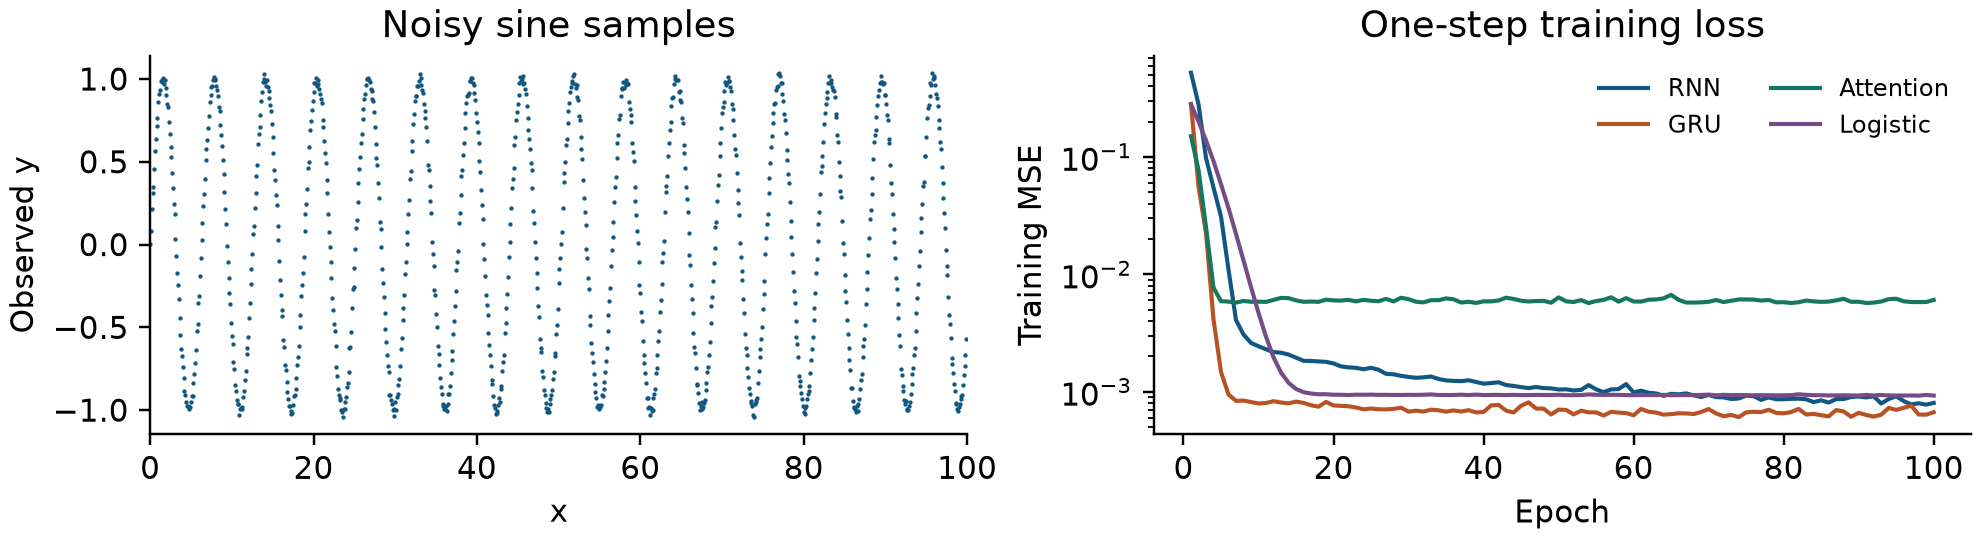
\includegraphics[width=\linewidth]{results/data_and_loss.png}
\end{center}

\newpage
\question{4(c). Predicting 200 steps ahead}
Each forecast starts with \(y_{991},\ldots,y_{1000}\) and feeds each prediction back into the window. The dashed line is the clean sine wave. The RNN keeps oscillating, but its peaks arrive early. Logistic regression drifts less over these 200 steps, while attention misses the oscillation.

\begin{center}
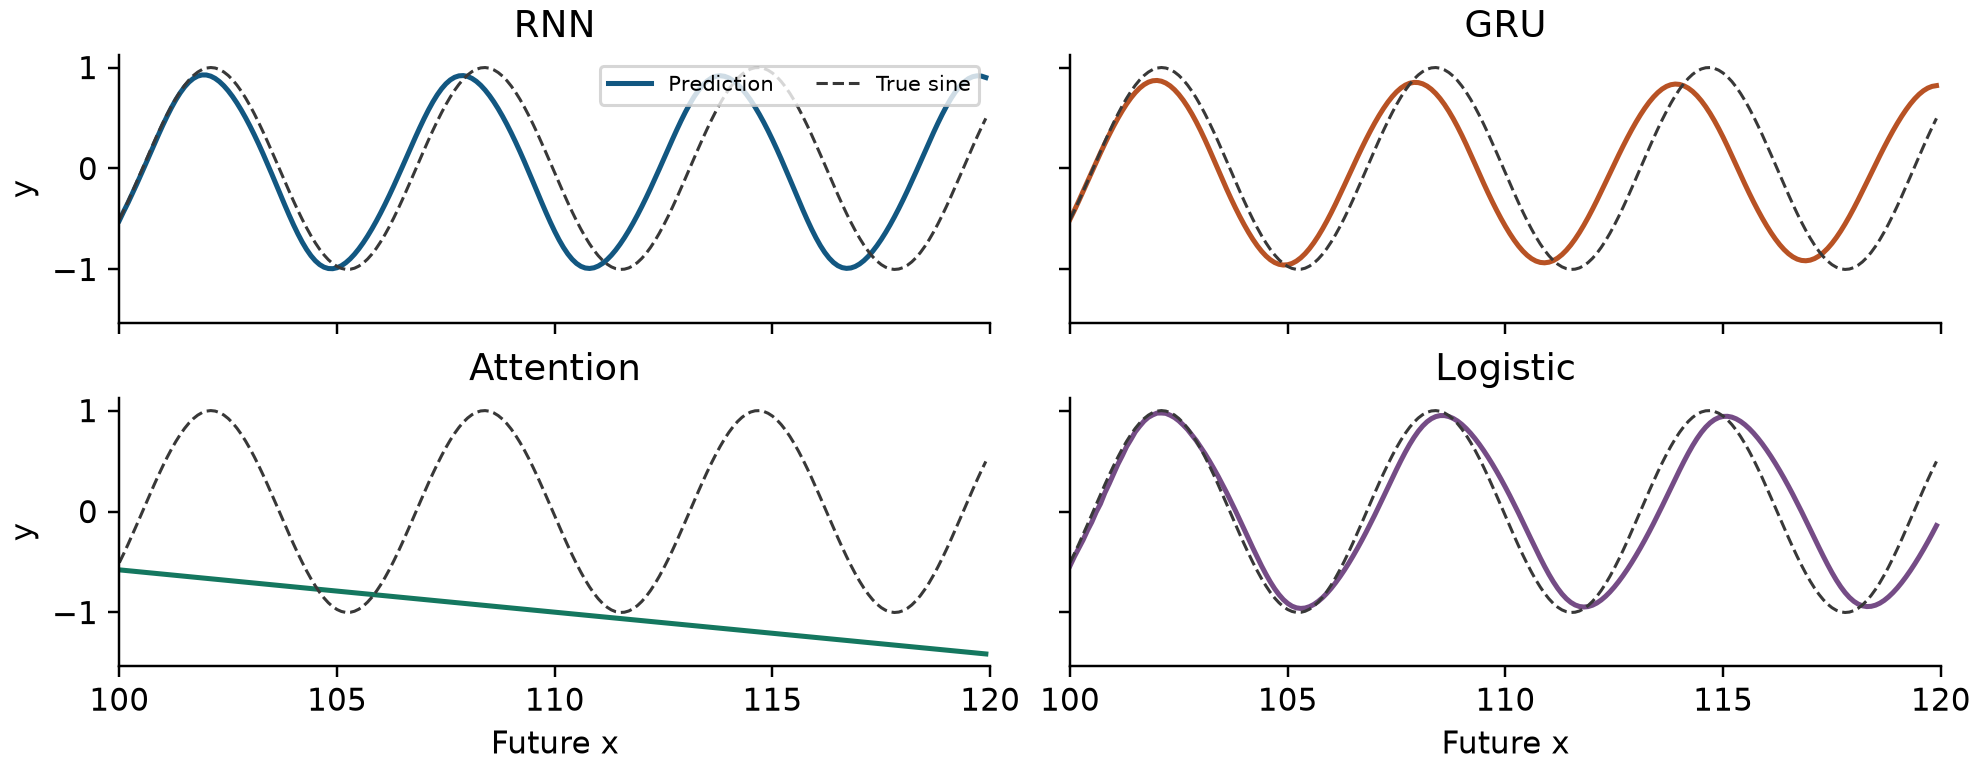
\includegraphics[width=.94\linewidth]{results/forecasts.png}\\[4pt]
\begin{tabular}{lrrr}
\toprule
Model & Final training MSE & Forecast RMSE & Time for 200 steps (ms)\\
\midrule
RNN       & 0.000801 & 0.471 & 9.35\\
GRU       & 0.000668 & 0.422 & 9.67\\
Attention & 0.006047 & 1.208 & 14.58\\
Logistic  & 0.000925 & 0.249 & 4.65\\
\bottomrule
\end{tabular}\\[3pt]
{\small RMSE is relative to the clean sine. Times are medians of five GPU runs after warm-up.}
\end{center}

\question{5. Paper summaries}
\paper{https://arxiv.org/abs/1609.02907}{Semi-Supervised Classification with Graph Convolutional Networks}
\textit{Motivation.} How can a citation network help classify papers when few have labels?\\
\textit{Novelty.} A first-order graph convolution mixes each node's features with its neighbors' features using degree-normalized weights. Training uses labels only where available.\\
\textit{Intuition.} Papers that cite each other often share a topic. A neighbor's words can help classify a paper whose own text gives little away.\\
\textit{Implementation.} \url{https://github.com/tkipf/gcn}

\paper{https://arxiv.org/abs/1710.10903}{Graph Attention Networks}
\textit{Motivation.} Some neighbors tell us more about a node's class than others.\\
\textit{Novelty.} Masked attention learns a score for each connected pair and normalizes the scores over the node's neighborhood.\\
\textit{Intuition.} A paper can give more weight to a citation on the same topic than to one it cites only for background.\\
\textit{Implementation.} \url{https://github.com/PetarV-/GAT}

\paper{https://arxiv.org/abs/1406.2661}{Generative Adversarial Networks}
\textit{Motivation.} Training deep generative models often required costly approximate inference.\\
\textit{Novelty.} A generator turns noise into samples. A discriminator learns to tell generated samples from real ones, and its feedback trains the generator.\\
\textit{Intuition.} If generated samples lack a feature common in real data, the discriminator can detect it. The generator then has a reason to learn that feature.\\
\textit{Implementation.} \url{https://github.com/goodfeli/adversarial}
\end{document}
